
\documentclass{article}
\usepackage[fontsize=14pt]{fontsize}

\usepackage{fontspec}
\setsansfont{CMU Sans Serif}
\setmainfont{CMU Serif}
\setmonofont{CMU Typewriter Text}

\defaultfontfeatures{Ligatures={TeX}}
\usepackage[english, ukrainian]{babel}
\usepackage[math-style=TeX]{unicode-math}
\usepackage{sidecap}
\sidecaptionvpos{figure}{c}

\usepackage[%
		a4paper,%
		footskip=1cm,%
		headsep=0.3cm,%
		top=2cm,%
		bottom=2cm,%
		left=2cm,%
		right=2cm]{geometry}

\usepackage{wrapstuff}
\usepackage{graphicx}
\graphicspath{{Pictures}}
\usepackage{caption}		
\pagestyle{empty}

		
\begin{document}
	
	
\begin{wrapstuff}[type=figure, l, top=4, width=0.42\linewidth]
	\centering
	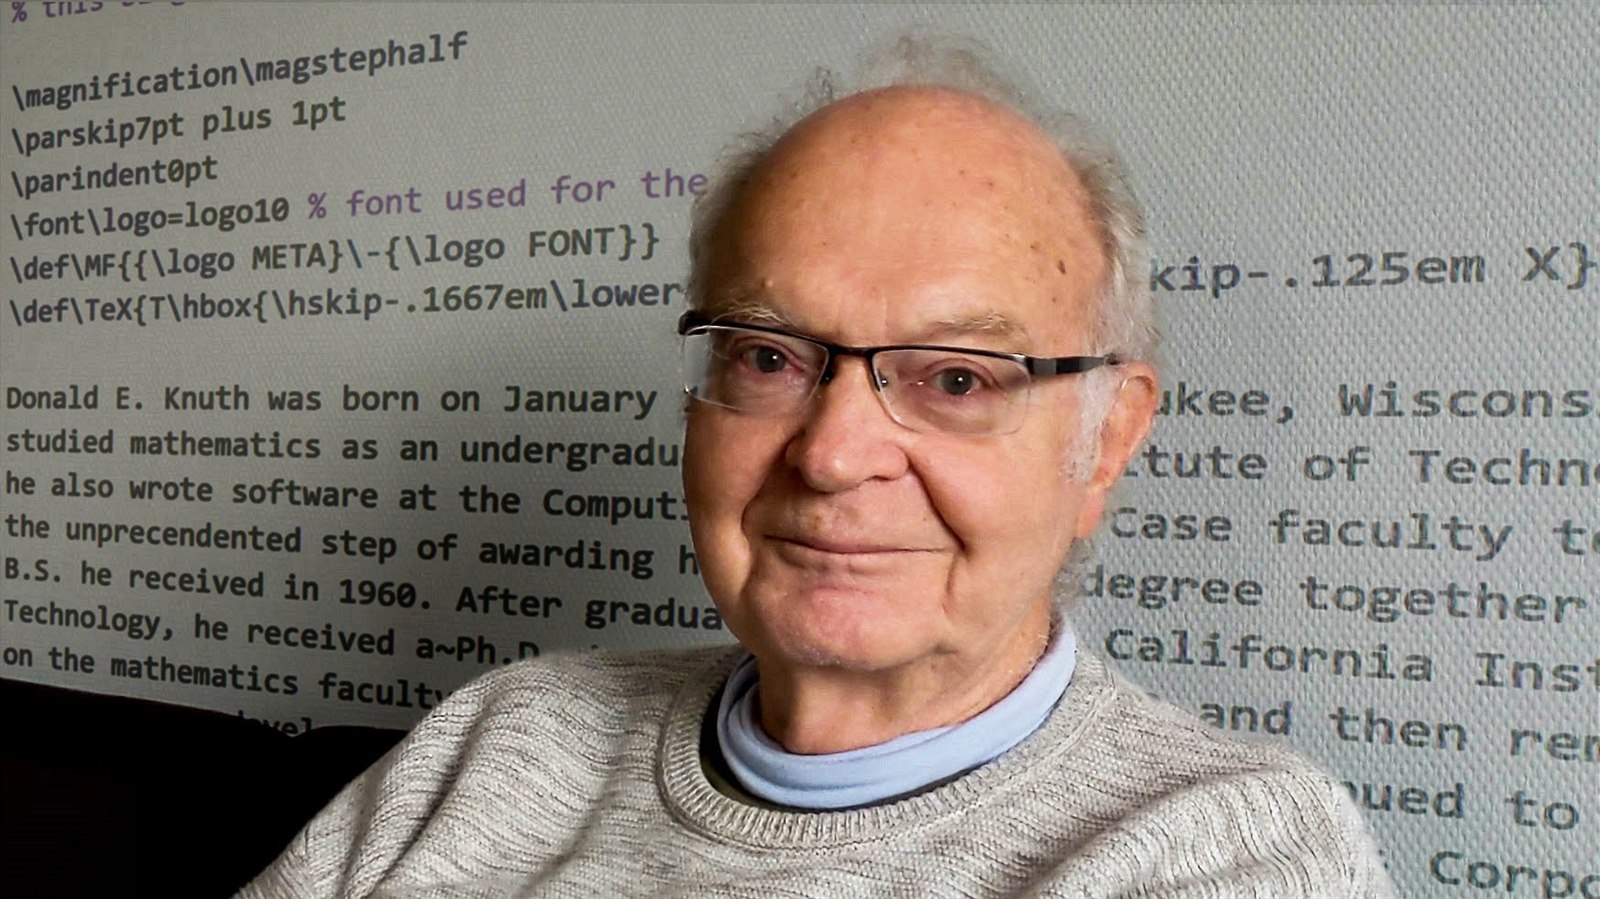
\includegraphics[width=\textwidth]{Knuth}
	\captionsetup{justification=centering}
	\caption{Дональд Ервін Кнут}
	\label{Knuth}
\end{wrapstuff}
Дональд Ервін Кнут (рис.~\ref{Knuth}) (10 січня 1938, Мілвокі, Вісконсин)~--- інформатик, ідеолог програмування та почесний професор Стенфордського університету. Автор фундаментальної праці \textit{«Мистецтво програмування»}; вважається одним з батьків аналізу складності алгоритмів. Розробник типографічної системи \TeX{}  та пов'язаної мови визначення шрифтів і системи їх рендерингу \texttt{METAFONT}.
	
	
Кнут народився у місті Мілвокі, штат Вісконсин, в сім'ї німецьких американців Генрі Кнута та Луізи Марії Бонінг. Батько Дональда працював на двох роботах: викладав бухгалтерію у Старшій Школі Мілвокі та вів невелике підприємство по друку. Молодший Кнут, навчаючись у тій же школі, отримав багато академічних відзнак, більшість з яких за геніальні способи вирішення різноманітних проблем. Наприклад, у восьмому класі він взяв участь у змаганні, в якому потрібно було відшукати всі слова, які можна скласти з букв словосполуки «Ziegler's Giant Bar». У суддейському списку було 2500 слів, та Дональду вдалось знайти 4500 та перемогти у конкурсі.
	
Освіта У 1956 році Кнут отримав запрошення до Технологічного Інституту (рис.~\ref{CWRU}) у Клівленді, Огайо, де вперше познайомився з \texttt{IBM 650}, одним із перших мейнфреймів. Прочитавши посібник до комп'ютера, Кнут вирішив переписати код компілятора для комп'ютера з його колишньої школи, тому що він вірив, що зможе зробити його краще.

\begin{SCfigure}[0.75][h]
	\centering
	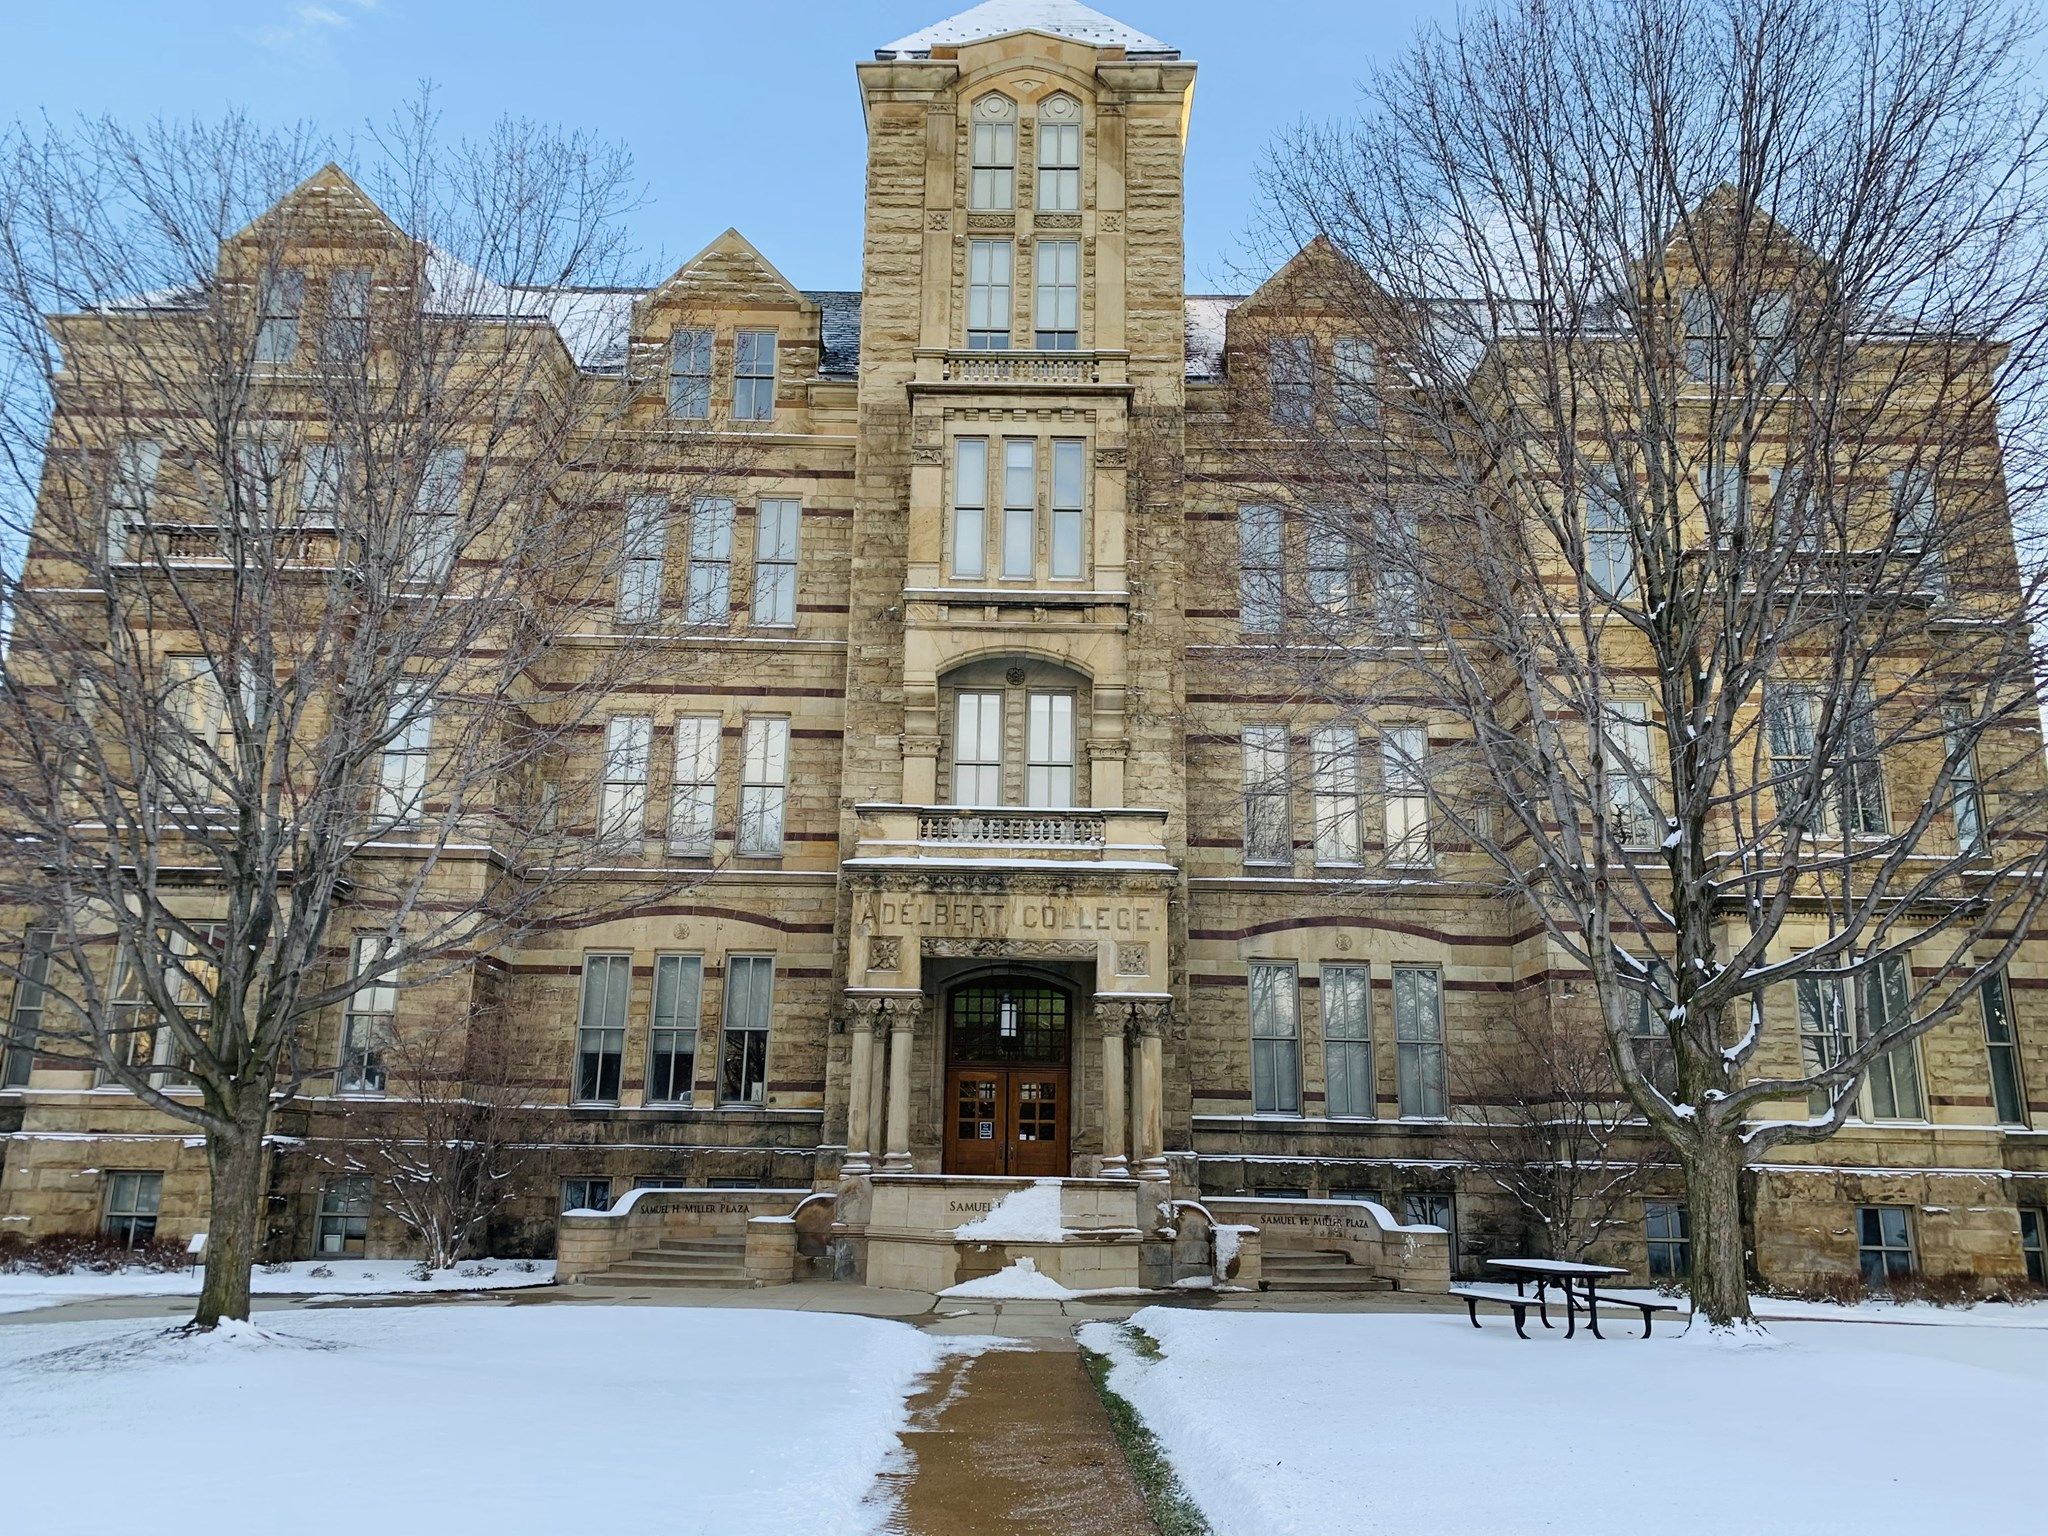
\includegraphics[width=0.5\textwidth]{CWRU}
	\caption{Західний резервний університет Кейса (CWRU)}
	\label{CWRU}
\end{SCfigure}
	
У 1958 році Кнут створив програму, щоб допомогти шкільній баскетбольній команді вигравати більше матчів. Він призначив кожному гравцю «вартість», щоб оцінити імовірність кожного баскетболіста здобути очки. Цей підхід оцінили видання Newsweek і CBS Evening News, згадавши Кнута у своїх випусках.
	
	
\end{document}